%%%%%%%%%%%%%%%%%%%%%%%%%%%%%%%%%%%%%%%%%
% Daily Laboratory Book
% LaTeX Template
%
% This template has been downloaded from:
% http://www.latextemplates.com
%
% Original author:
% Frank Kuster (http://www.ctan.org/tex-archive/macros/latex/contrib/labbook/)
%
% Important note:
% This template requires the labbook.cls file to be in the same directory as the
% .tex file. The labbook.cls file provides the necessary structure to create the
% lab book.
%
% The \lipsum[#] commands throughout this template generate dummy text
% to fill the template out. These commands should all be removed when 
% writing lab book content.
%
% HOW TO USE THIS TEMPLATE 
% Each day in the lab consists of three main things:
%
% 1. LABDAY: The first thing to put is the \labday{} command with a date in 
% curly brackets, this will make a new page and put the date in big letters 
% at the top.
%
% 2. EXPERIMENT: Next you need to specify what experiment(s) you are 
% working on with an \experiment{} command with the experiment shorthand 
% in the curly brackets. The experiment shorthand is defined in the 
% 'DEFINITION OF EXPERIMENTS' section below, this means you can 
% say \experiment{pcr} and the actual text written to the PDF will be what 
% you set the 'pcr' experiment to be. If the experiment is a one off, you can 
% just write it in the bracket without creating a shorthand. Note: if you don't 
% want to have an experiment, just leave this out and it won't be printed.
%
% 3. CONTENT: Following the experiment is the content, i.e. what progress 
% you made on the experiment that day.
%
%%%%%%%%%%%%%%%%%%%%%%%%%%%%%%%%%%%%%%%%%

%----------------------------------------------------------------------------------------
%	PACKAGES AND OTHER DOCUMENT CONFIGURATIONS
%----------------------------------------------------------------------------------------

\documentclass[hyperref,openany,10pt]{labbook} % 'openany' here removes the gap page between days, erase it to restore this gap; 'oneside' can also be added to remove the shift that odd pages have to the right for easier reading

\usepackage[ 
  backref=page,
  pdfpagelabels=true,
  plainpages=false,
  colorlinks=true,
  bookmarks=true,
  pdfview=FitB]{hyperref} % Required for the hyperlinks within the PDF
  
\usepackage[utf8]{inputenc} % Required for the top and bottom rules in the table
\usepackage[T1]{fontenc} % Required for the top and bottom rules in the table
\usepackage[french]{babel} % Required for the top and bottom rules in the table
\usepackage{booktabs} % Required for the top and bottom rules in the table
\usepackage{float} % Required for specifying the exact location of a figure or table
\usepackage{graphicx} % Required for including images
\usepackage{lipsum} % Used for inserting dummy 'Lorem ipsum' text into the template
\usepackage{grffile} % changes the algorithm to check for known extensions (option multidot, enabled by default)
\usepackage{subfigure} % Allow subfigure with their own caption
\usepackage{xcolor}
\definecolor{bl}{rgb}{0.0,0.2,0.6} 
\usepackage{sectsty}
\usepackage[title,titletoc,toc]{appendix}
\usepackage[compact]{titlesec}
\allsectionsfont{\color{bl}\scshape\selectfont}
\renewcommand{\sectfont}{\color{bl}\scshape\selectfont}

\newcommand{\HRule}{\rule{\linewidth}{0.5mm}} % Command to make the lines in the title page
\setlength\parindent{0pt} % Removes all indentation from paragraphs

%----------------------------------------------------------------------------------------
%	DEFINITION OF EXPERIMENTS
%----------------------------------------------------------------------------------------

\newexperiment{example}{This is an example experiment}
\newexperiment{example2}{This is another example experiment}
\newexperiment{example3}{This is yet another example experiment}
\newexperiment{table}{This shows a sample table}
%\newexperiment{shorthand}{Description of the experiment}

%---------------------------------------------------------------------------------------

\begin{document}

%----------------------------------------------------------------------------------------
%	TITLE PAGE
%----------------------------------------------------------------------------------------

\frontmatter % Use Roman numerals for page numbers
\title{
\begin{center}
\HRule \\[0.4cm]
{\Huge \bfseries Cahier d'expérience \\[0.5cm] \Large Master de Science des Données}\\[0.4cm] % Degree
\HRule \\[1.5cm]
\end{center}
}
\author{\Huge Victor Estrade \\ \\ \LARGE victor.estrade@u-psud.fr \\[2cm]} % Your name and email address
\date{Début $1^{er}$ Avril 2016} % Beginning date
\maketitle

\tableofcontents

\mainmatter % Use Arabic numerals for page numbers

%----------------------------------------------------------------------------------------
%	LAB BOOK CONTENTS
%----------------------------------------------------------------------------------------


\labday{Mardi, 5 avril 2016}

Expérimentation sur le correcteur. Je vais résumé ici mes résultats et remarques
sur l'utilisation d'un correcteur simple (une seule couche) pour apprendre par l'exemple
à inverser des transformations linéaires simples.

Pour ce j'utilise le modèle simpliste (figure \ref{fig:correcteur}). 
Sans utilisation d'adversarial.

\begin{figure}[H] % Example of including images
\centering
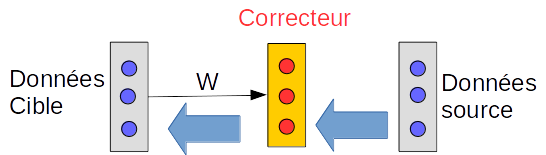
\includegraphics[width=0.45\linewidth]{fig/05-04-2016/Correcteur.png}
\caption{Correcteur simple}
\label{fig:correcteur}
\end{figure}

Le réseau est entraîné par minibatch avec un nombre d'époque prédéfini à la main.
La fonction de coût utilisée est la \emph{mean squared error} : $(x_{pred}-x_{vrai})^2$

Puisqu'il n'y a pas de \emph{décodeur} l'unique couche (unique matrice de poids $W$)
est constituée de $d$ neurone où $d$ est le nombre de descripteur des données.


\experiment{Corriger MNIST après transformations linéaires}

Dans un premier temps sur MNIST.
Le réseaux doit reconstruire l'image transformée.
MNIST est assez pratique car il permet de visualiser facilement l'efficacité 
de la reconstruction pour des données avec un bon nombre de descripteurs (748 pixels).

\subexperiment{Alignées}

Tout d'abord j'ai gardé la correspondance entre l'image original et
l'image transformée pendant l'entraînement du correcteur (cas aligné).
Ainsi chaque paire d'exemple $(x, \phi(x)) \in MNIST\times \phi(MNIST)$
contient uniquement l'information que l'on cherche $\phi$.

Ce qui donne de très bon résultats la plupart du temps.\\


{\Large\textbf{Mirror.}} On commence par une simple permutation des 
descripteurs de façon à renverser les images.

Le correcteur se débrouille sans souci, sans avoir besoin d'adversarial. Ceci
nous offre un exemple typique de cas où tout se passe bien. Les résultats sont résumés
figure \ref{fig:mnist_mirror_pairwise}.

\begin{figure}[H] % Example of including images
\centering
\subfigure[Sample images]
	{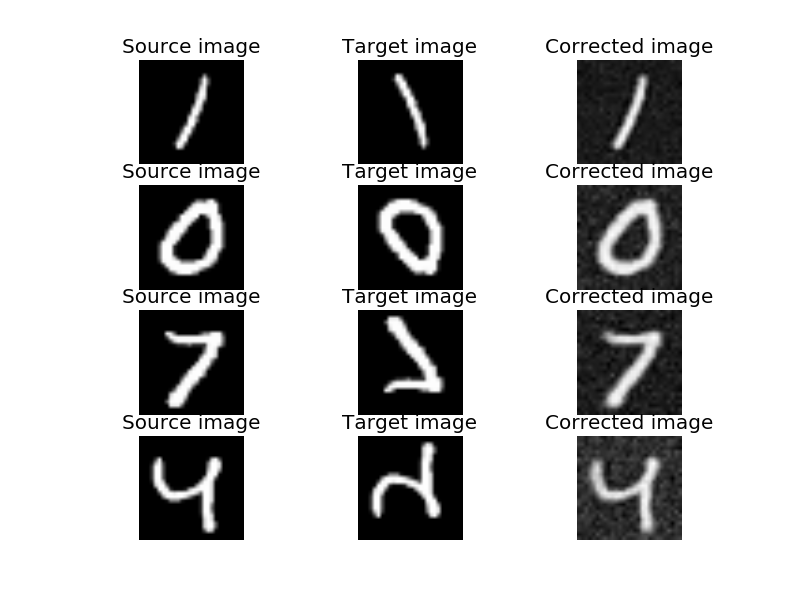
\includegraphics[width=0.45\linewidth]{fig/05-04-2016/MNISTMirror-PairWiseCorrector-lambda-0.0000-sample.png}}
\hfill
\subfigure[Learning curve (squared loss)]
	{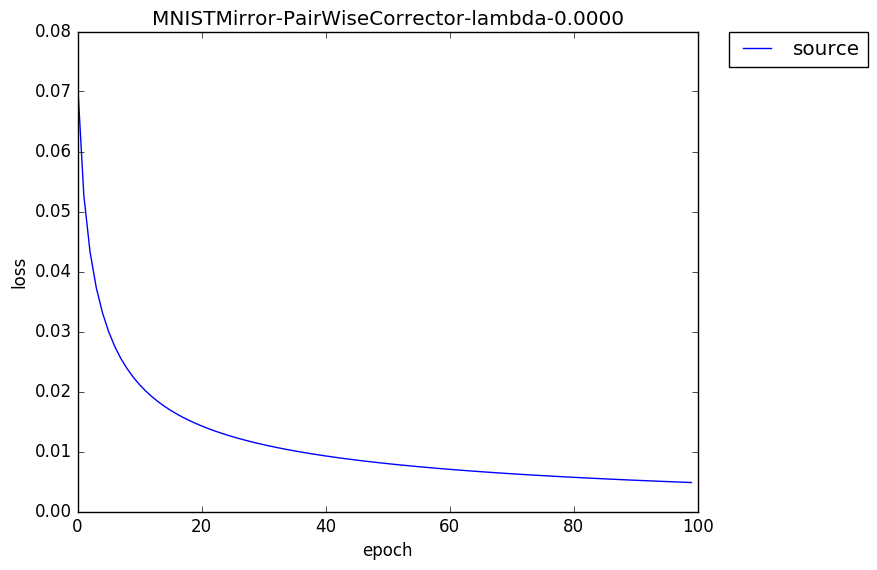
\includegraphics[width=0.45\linewidth]{fig/05-04-2016/MNISTMirror-PairWiseCorrector-lambda-0.0000.png}}
\subfigure[Weights]
	{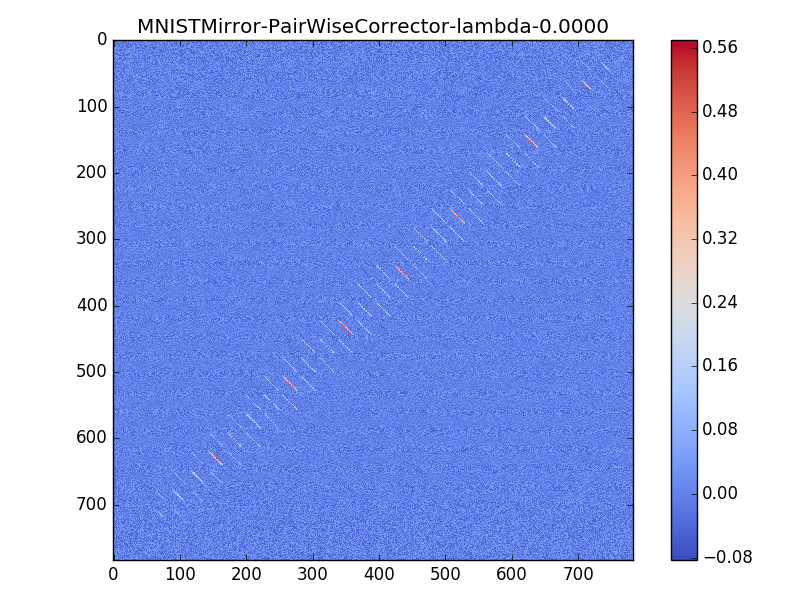
\includegraphics[width=0.45\linewidth]{fig/05-04-2016/MNISTMirror-PairWiseCorrector-lambda-0.0000-Weights.png}}
\caption{MNIST - Mirror correcteur aligné}
\label{fig:mnist_mirror_pairwise}
\end{figure}


{\Large\textbf{RMat.}} On se lance maintenant dans un problème légèrement plus
difficile pour la machine mais impossible pour l'œil humain, une transformation
linéaire aléatoire:
$$ \phi(x) = A.x$$
où $A$ est une matrice générée aléatoirement.

Pour éviter les problèmes d'échelle, les données ont été renormalisées après 
transformation (sinon : loss = NaN).

Les résultats sur cette transformation sont assez mitigés. De plus elle requiert
un entraînement particulièrement long (quelques centaines d'époques). Mais bon avec
les yeux de la fois et en choisissant les bons exemples ça a l'air de fonctionner.
Une fois de plus les résultats sont résumés figure \ref{fig:mnist_rmat_pairwise}.

\begin{figure}[H] % Example of including images
\centering
\subfigure[Sample images]
	{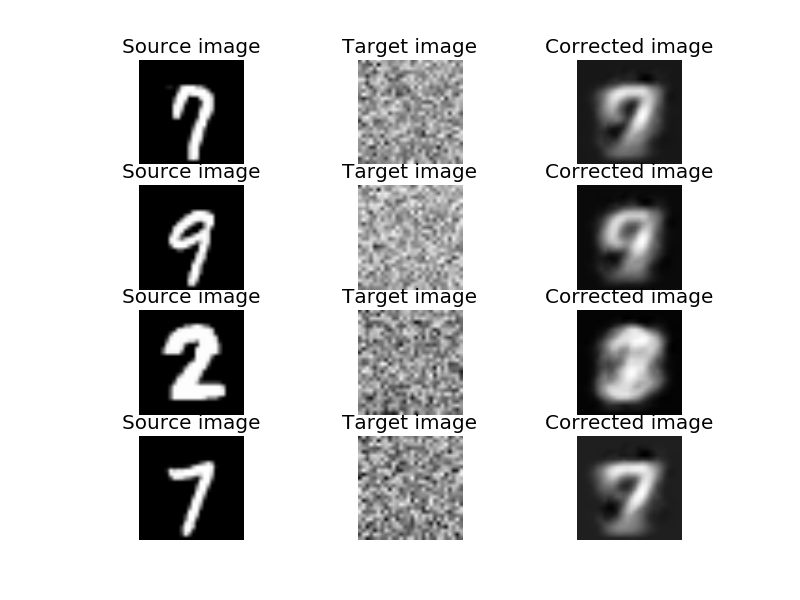
\includegraphics[width=0.45\linewidth]{fig/05-04-2016/MNISTRMat-PairWiseCorrector-lambda-0.0000-sample.png}}
\hfill
\subfigure[Learning curve (squared loss)]
	{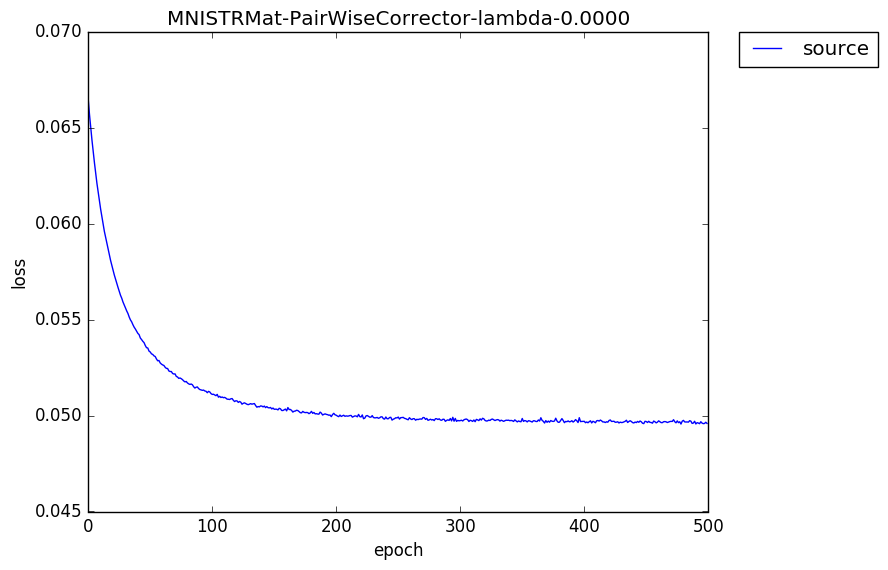
\includegraphics[width=0.45\linewidth]{fig/05-04-2016/MNISTRMat-PairWiseCorrector-lambda-0.0000.png}}
\subfigure[Weights]
	{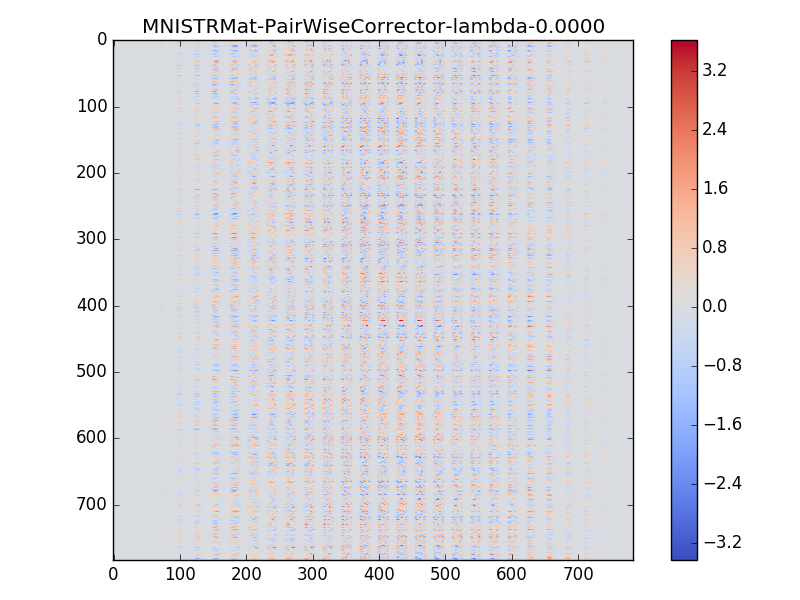
\includegraphics[width=0.45\linewidth]{fig/05-04-2016/MNISTRMat-PairWiseCorrector-lambda-0.0000-Weights.png}}
\caption{MNIST - RMat correcteur aligné}
\label{fig:mnist_rmat_pairwise}
\end{figure}


\subexperiment{Non alignées}

Ici chaque paire d'exemple $(x_i, \phi(x_j)) \in MNIST\times \phi(MNIST)$
ne contient pas uniquement l'information que l'on cherche $\phi$. Même si
les exemples $x_i$ et $x_j$ sont choisis parmi la même classe, ces exemples 
se différencient non seulement par la transformation subie mais aussi par 
les variations au sein d'une même classes.

Ceci est plus proche de cas d'expériences réels. Exemple: des échantillons
du même type sans être exactement les mêmes et utilisant des instruments
de précision différents.

L'entraînement est donc légèrement plus complexe. Pour le moment j'ai utilisé 
la version naïve où je sélectionne aléatoirement les exemples d'une même classe
pour être alignés. Cette sélection change à chaque nouvelle époque. Des 
améliorations possibles de cette technique seront développées plus loin.\\


{\Large\textbf{Mirror.}} à nouveau l'on commence par le cas simple des images 
miroirs. Cette fois ci la qualité des résultats est plus discutable. 

\begin{figure}[H] % Example of including images
\centering
\subfigure[Sample images]
	{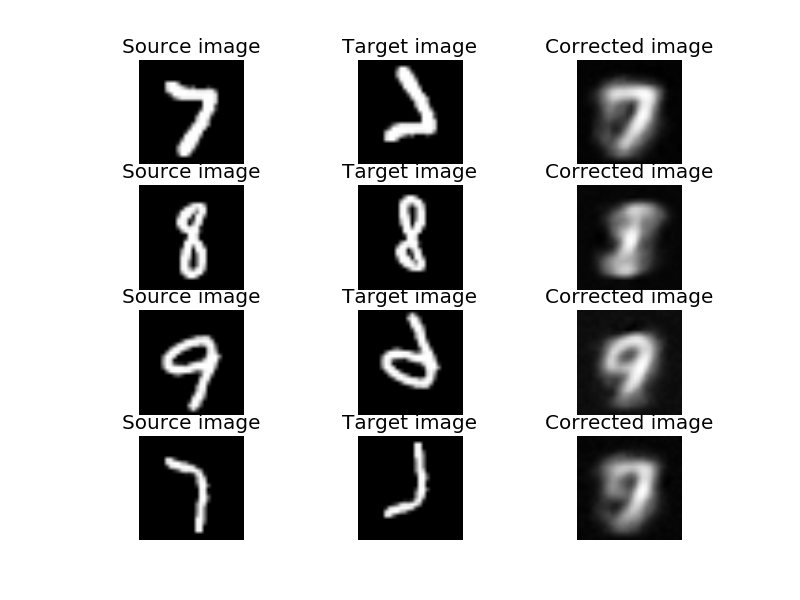
\includegraphics[width=0.45\linewidth]{fig/05-04-2016/MNISTMirror-ClassWiseCorrector-lambda-0.0000-sample.png}}
\hfill
\subfigure[Learning curve (squared loss)]
	{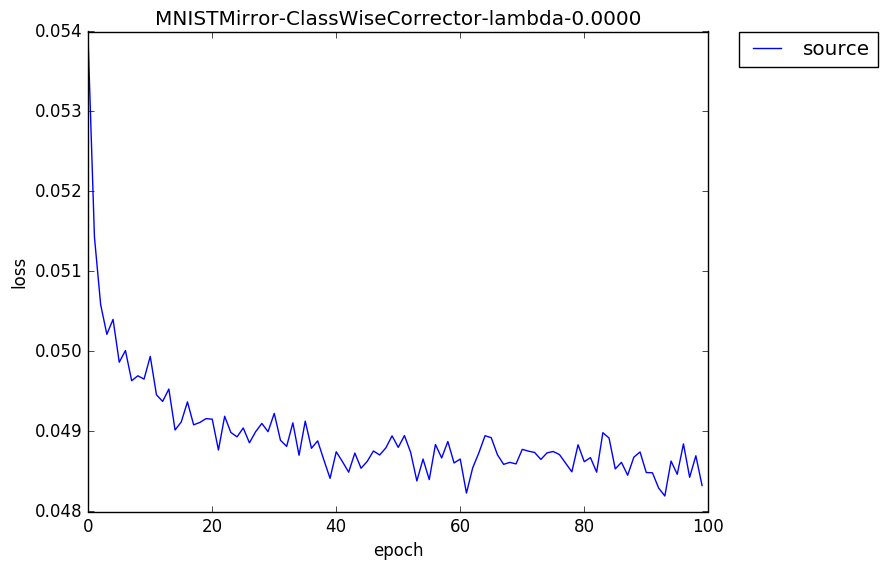
\includegraphics[width=0.45\linewidth]{fig/05-04-2016/MNISTMirror-ClassWiseCorrector-lambda-0.0000.png}}
\subfigure[Weights]
	{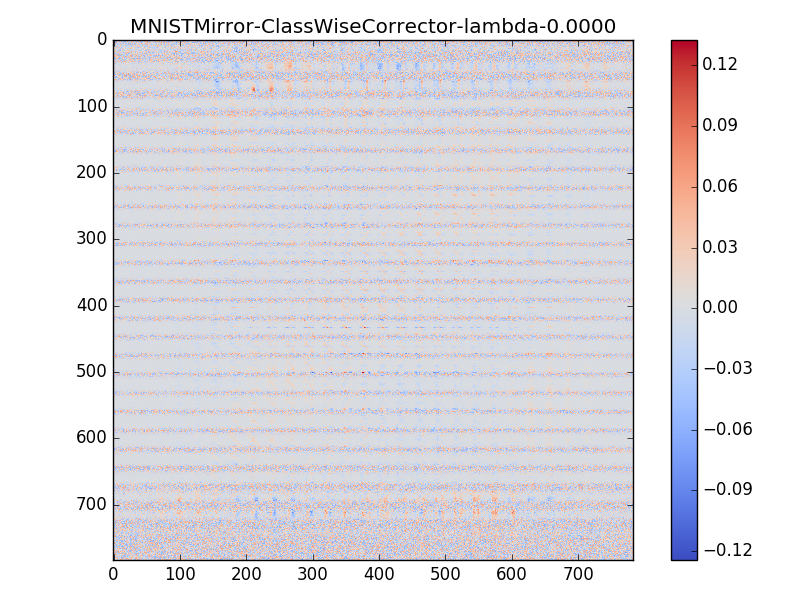
\includegraphics[width=0.45\linewidth]{fig/05-04-2016/MNISTMirror-ClassWiseCorrector-lambda-0.0000-Weights.png}}
\caption{MNIST - Mirror correcteur non aligné}
\label{fig:mnist_mirror_classwise}
\end{figure}


{\Large\textbf{RMat.}} On reprend la transformation linéaire aléatoire:
$$ \phi(x) = A.x$$
où $A$ est une matrice générée aléatoirement.


\begin{figure}[H] % Example of including images
\centering
\subfigure[Sample images]
	{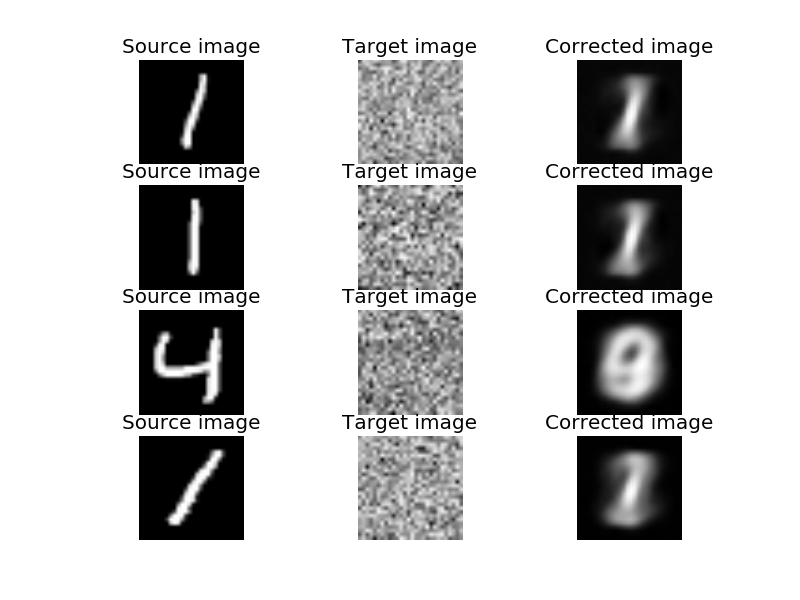
\includegraphics[width=0.45\linewidth]{fig/05-04-2016/MNISTRMat-ClassWiseCorrector-lambda-0.0000-sample.png}}
\hfill
\subfigure[Learning curve (squared loss)]
	{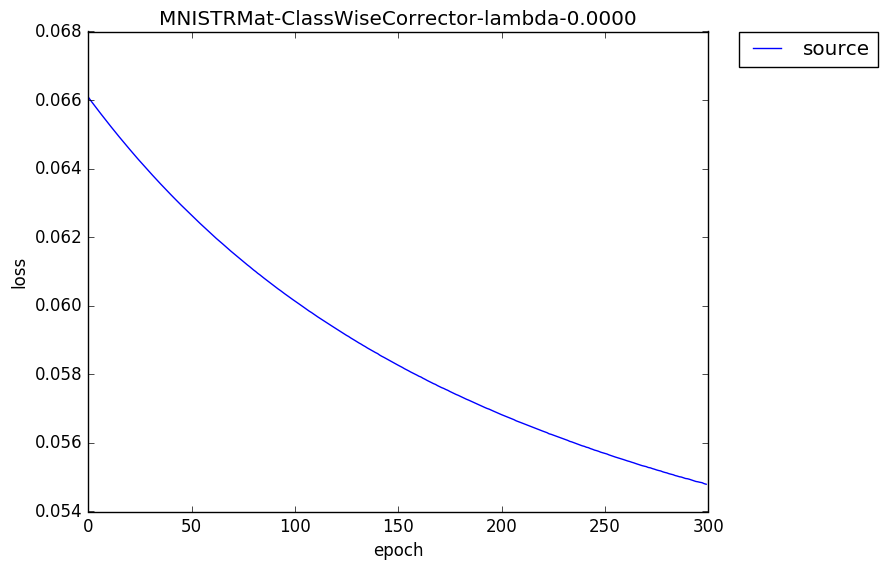
\includegraphics[width=0.45\linewidth]{fig/05-04-2016/MNISTRMat-ClassWiseCorrector-lambda-0.0000.png}}
\subfigure[Weights]
	{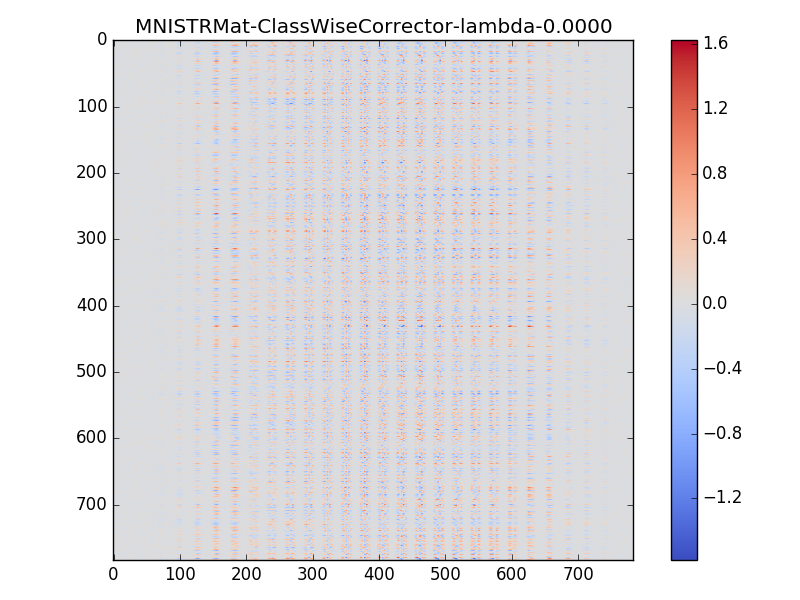
\includegraphics[width=0.45\linewidth]{fig/05-04-2016/MNISTRMat-ClassWiseCorrector-lambda-0.0000-Weights.png}}
\caption{MNIST - RMat correcteur non aligné}
\label{fig:mnist_rmat_classwise}
\end{figure}


%-----------------------------------------

\experiment{Corriger Moon après transformations linéaire}

Maintenant on passe sur des données à 2 dimensions. L'exemple des demi-lunes
(Moon) est un exemple non linéaire simple en 2D.

%----------------------------------------------------------------------------------------

%----------------------------------------------------------------------------------------


%----------------------------------------------------------------------------------------

%----------------------------------------------------------------------------------------
%	FORMULAE AND MEDIA RECIPES
%----------------------------------------------------------------------------------------

\labday{} % We don't want a date here so we make the labday blank

\begin{center}
\HRule \\[0.4cm]
{\huge \textbf{Jolie titre !}}\\[0.4cm] % Heading
\HRule \\[1.5cm]
\end{center}

%----------------------------------------------------------------------------------------
%	FORMULAE
%----------------------------------------------------------------------------------------

\newpage

\huge \textbf{Formulae} \\ \\

\normalsize \textbf{Formula 1 - Pythagorean theorem}\\ \\
$a^2 + b^2 = c^2$\\ \\

%-----------------------------------------

%\textbf{Formula X - Description}\\ \\

%Formula

%----------------------------------------------------------------------------------------

\end{document}